\documentclass[11pt,a4paper,oneside]{article}\usepackage[]{graphicx}\usepackage[]{color}
%% maxwidth is the original width if it is less than linewidth
%% otherwise use linewidth (to make sure the graphics do not exceed the margin)
\makeatletter
\def\maxwidth{ %
  \ifdim\Gin@nat@width>\linewidth
    \linewidth
  \else
    \Gin@nat@width
  \fi
}
\makeatother

\definecolor{fgcolor}{rgb}{0.345, 0.345, 0.345}
\newcommand{\hlnum}[1]{\textcolor[rgb]{0.686,0.059,0.569}{#1}}%
\newcommand{\hlstr}[1]{\textcolor[rgb]{0.192,0.494,0.8}{#1}}%
\newcommand{\hlcom}[1]{\textcolor[rgb]{0.678,0.584,0.686}{\textit{#1}}}%
\newcommand{\hlopt}[1]{\textcolor[rgb]{0,0,0}{#1}}%
\newcommand{\hlstd}[1]{\textcolor[rgb]{0.345,0.345,0.345}{#1}}%
\newcommand{\hlkwa}[1]{\textcolor[rgb]{0.161,0.373,0.58}{\textbf{#1}}}%
\newcommand{\hlkwb}[1]{\textcolor[rgb]{0.69,0.353,0.396}{#1}}%
\newcommand{\hlkwc}[1]{\textcolor[rgb]{0.333,0.667,0.333}{#1}}%
\newcommand{\hlkwd}[1]{\textcolor[rgb]{0.737,0.353,0.396}{\textbf{#1}}}%

\usepackage{framed}
\makeatletter
\newenvironment{kframe}{%
 \def\at@end@of@kframe{}%
 \ifinner\ifhmode%
  \def\at@end@of@kframe{\end{minipage}}%
  \begin{minipage}{\columnwidth}%
 \fi\fi%
 \def\FrameCommand##1{\hskip\@totalleftmargin \hskip-\fboxsep
 \colorbox{shadecolor}{##1}\hskip-\fboxsep
     % There is no \\@totalrightmargin, so:
     \hskip-\linewidth \hskip-\@totalleftmargin \hskip\columnwidth}%
 \MakeFramed {\advance\hsize-\width
   \@totalleftmargin\z@ \linewidth\hsize
   \@setminipage}}%
 {\par\unskip\endMakeFramed%
 \at@end@of@kframe}
\makeatother

\definecolor{shadecolor}{rgb}{.97, .97, .97}
\definecolor{messagecolor}{rgb}{0, 0, 0}
\definecolor{warningcolor}{rgb}{1, 0, 1}
\definecolor{errorcolor}{rgb}{1, 0, 0}
\newenvironment{knitrout}{}{} % an empty environment to be redefined in TeX

\usepackage{alltt}
\usepackage{amsmath,amsthm,amsfonts,amssymb}
\usepackage{pst-eucl,pstricks,pstricks-add}
%\usepackage[utf8]{inputenc}
%\usepackage[latin1]{inputenc}
\usepackage[spanish,activeacute]{babel}
\usepackage[a4paper,margin=2.5cm]{geometry}
\usepackage{times}
\usepackage[T1]{fontenc}
\usepackage{titlesec}
\usepackage{color}
\usepackage{url}
\usepackage{float}
\usepackage{cite}
\usepackage{graphicx}
\usepackage{multicol}
\usepackage{float}
\usepackage{lmodern}
\parindent=0mm
\IfFileExists{upquote.sty}{\usepackage{upquote}}{}
\begin{document}

\thispagestyle{empty}
{\sf
{\Large \scshape Escuela Polit\'{e}cnica Nacional} \hfill {\scshape 24 de Febrero 2016}\\[3mm] 
{\scshape C\'{a}lculo en una variable \hfill Examen Supletorio}\\[7mm]
{\scshape Nombre:} \rule{0.6\textwidth}{0.5pt}\qquad {\scshape Nro. lista:} \rule{0.1\textwidth}{0.5pt}\\
}




\begin{enumerate}
      \item Usando la definición de límite muestre que: $\displaystyle \lim_{x \to -5} \frac{3x^2+22x+40}{2x^2+13x+21}=\frac{5}{6}$
      
      \item Calcule el siguiente límite: $\displaystyle \lim_{x\to +\infty} \sqrt{5x-4\sqrt{x}+1}-\sqrt{5x+3\sqrt{x}-2} $
      
      \item Encuentre la derivada de la función: $\displaystyle f(x)=\sqrt{4x}\ (x^{-3}+1)^5 e^{x^2}$
      
      \item Halle $f'(x)$ empleando el teorema de la función inversa de: $f(x)=\arcsin \displaystyle\frac{x}{2}$
      
      \item Encuentre $\displaystyle \frac{dy}{dx}$ si $xy^2 +\sen(y) \ln xy + x^3y^2=\displaystyle \frac{x}{y}$
      
      \item Hallar la base B y la altura H de una cartulina en forma rectangular de 60 cm de perímetro, que, al dar la vuelta completa alrededor de un lado vertical, genera un cilindro de volumen máximo.
      
      \begin{figure}[H]
      \centering
      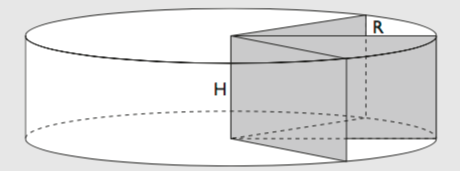
\includegraphics[scale=0.45]{derivada.png}
      \end{figure}
      
      \item Encuentre $\displaystyle \int_{-1}^{4} f(x) dx$, conocido que $\displaystyle \int_{-1}^{4} \left[2f(x)-7\right]\ dx=-31$.
      
      \item Calcule las siguientes integrales: 
      \begin{enumerate}
            \item $\displaystyle \int \frac{\ln \left(\ln x\right)}{x}\ dx$
            \item $\displaystyle \int \frac{x}{(x+1)(x^2+1)^2}\ dx$
            \item $\displaystyle \int \frac{x^2}{\sqrt{x^2+4x-12}}\ dx$
      \end{enumerate}
      
      \item Evalúe la siguiente integral impropia: $\displaystyle \int_{-\infty}^{+\infty} \frac{dx}{e^x+e^{-x}}$
      
      \item Calcule el volumen del sólido que genera la región limitada por las curvas: $y=2(x-2)^2$; $y=2x$, cuando rota alrededor del eje $x=-1$.

\end{enumerate}

\end{document}
